\chapter{The S-matrix and physical observables}

\section{Decay Rate}
Consider the case in which the initial state is a single particle and the final state is given by n particles. We are therefore considering a decay process. Assume for the moment that particles are indistinguishable.

\begin{center}
\tikzset{every picture/.style={line width=0.75pt}} %set default line width to 0.75pt        
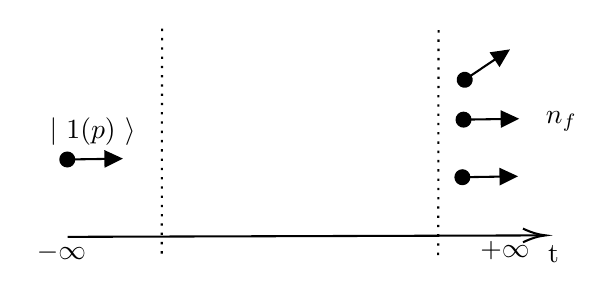
\begin{tikzpicture}[x=0.75pt,y=0.75pt,yscale=-1,xscale=1]
%uncomment if require: \path (0,194); %set diagram left start at 0, and has height of 194

%Straight Lines [id:da28910037002363764] 
\draw    (205.27,107.68) -- (433.59,106.98) ;
\draw [shift={(435.59,106.97)}, rotate = 539.8199999999999] [color={rgb, 255:red, 0; green, 0; blue, 0 }  ][line width=0.75]    (10.93,-3.29) .. controls (6.95,-1.4) and (3.31,-0.3) .. (0,0) .. controls (3.31,0.3) and (6.95,1.4) .. (10.93,3.29)   ;
%Straight Lines [id:da7985070919800723] 
\draw  [dash pattern={on 0.84pt off 2.51pt}]  (250.78,7.4) -- (250.61,116.64) ;
%Straight Lines [id:da47959589803581304] 
\draw  [dash pattern={on 0.84pt off 2.51pt}]  (383.98,8.11) -- (383.81,117.35) ;
%Straight Lines [id:da17940445023321017] 
\draw    (205.1,70.41) -- (228.91,70.04) ;
\draw [shift={(231.91,69.99)}, rotate = 539.0899999999999] [fill={rgb, 255:red, 0; green, 0; blue, 0 }  ][line width=0.08]  [draw opacity=0] (8.93,-4.29) -- (0,0) -- (8.93,4.29) -- cycle    ;
\draw [shift={(205.1,70.41)}, rotate = 359.09] [color={rgb, 255:red, 0; green, 0; blue, 0 }  ][fill={rgb, 255:red, 0; green, 0; blue, 0 }  ][line width=0.75]      (0, 0) circle [x radius= 3.35, y radius= 3.35]   ;
%Straight Lines [id:da9397044962896224] 
\draw    (396.57,32.01) -- (415.9,19.03) ;
\draw [shift={(418.39,17.36)}, rotate = 506.11] [fill={rgb, 255:red, 0; green, 0; blue, 0 }  ][line width=0.08]  [draw opacity=0] (8.93,-4.29) -- (0,0) -- (8.93,4.29) -- cycle    ;
\draw [shift={(396.57,32.01)}, rotate = 326.11] [color={rgb, 255:red, 0; green, 0; blue, 0 }  ][fill={rgb, 255:red, 0; green, 0; blue, 0 }  ][line width=0.75]      (0, 0) circle [x radius= 3.35, y radius= 3.35]   ;
%Straight Lines [id:da4306245684857515] 
\draw    (395.46,78.95) -- (419.27,78.57) ;
\draw [shift={(422.27,78.52)}, rotate = 539.0899999999999] [fill={rgb, 255:red, 0; green, 0; blue, 0 }  ][line width=0.08]  [draw opacity=0] (8.93,-4.29) -- (0,0) -- (8.93,4.29) -- cycle    ;
\draw [shift={(395.46,78.95)}, rotate = 359.09] [color={rgb, 255:red, 0; green, 0; blue, 0 }  ][fill={rgb, 255:red, 0; green, 0; blue, 0 }  ][line width=0.75]      (0, 0) circle [x radius= 3.35, y radius= 3.35]   ;
%Straight Lines [id:da8816879387506134] 
\draw    (396.02,51.21) -- (419.83,50.83) ;
\draw [shift={(422.83,50.78)}, rotate = 539.0899999999999] [fill={rgb, 255:red, 0; green, 0; blue, 0 }  ][line width=0.08]  [draw opacity=0] (8.93,-4.29) -- (0,0) -- (8.93,4.29) -- cycle    ;
\draw [shift={(396.02,51.21)}, rotate = 359.09] [color={rgb, 255:red, 0; green, 0; blue, 0 }  ][fill={rgb, 255:red, 0; green, 0; blue, 0 }  ][line width=0.75]      (0, 0) circle [x radius= 3.35, y radius= 3.35]   ;


% Text Node
\draw (443.19,51.92) node    {$n_{f}$};
% Text Node
\draw (217.31,56.9) node    {$|\ 1( p) \ \rangle $};
% Text Node
\draw (439.31,115.93) node   [align=left] {t};
% Text Node
\draw (202.32,115.22) node    {$-\infty $};
% Text Node
\draw (416,114.51) node    {$+\infty $};

\end{tikzpicture}
\end{center}

The rules of quantum mechanics tell us that the probability for this process is obtained by taking the squared modulus of the amplitude and summing over all possible final states
\[
\begin{split}
\abs{S_{fi}^{CN}}^2	& = \abs{(2 \pi)^4 \delta^4 (p - p')M_{fi}^{CN}}^2 \\
				& = (2 \pi)^4 \delta^4 (p - p') (VT) \abs{M_{fi}^{CN}}^2 \\
				& = (2 \pi)^4 \delta^4 (p - p')(VT) \frac{1}{2 \omega_in V}
					\prod_{l=1}^{n_f} \biggl( \frac{1}{2 \omega_l V} \biggr) \abs{\mathM_{fi}}^2
\end{split}
\]
\textbf{Note:} $\bigl( \delta^4 (p - p') \bigr)^2 = \delta^4 (p - p') \delta^4 (p - p') = \delta^4 (p - p') \delta^4(0) = \delta^4 (p - p') \frac{VT}{(2 \pi)^4}$\\
We use the final space and time in order to remove divergent terms during calculation\\ \\
We must now sum this expression over all final states. Since we are working in a finite volume V, this is the sum over the possible discrete values of the momenta of the final particles .\\
Since $p_i = (2 \pi/L) n_i$, we have $dn_i = (L/2\pi) \de p_i$ and $\de^3 n_i = (V/(2 \pi)^3) \de^3 p$ where $\de^3 n_i$ is the infinitesimal phase space related to a final state in which the i-th particle has momentum between $p_i$ and $p_i + \de p_i$\\
Let $\de \omega$ be the probability for a decay in which in the final state the i-th particle has momentum between $p_i$ and $p_i \de p_i$
\[
\de \omega = \abs{S_{fi}^{SN}}^2 \prod_{l=1}^{n_f} \biggl( \frac{V\de^3 p_l}{(2 \pi)^3} \biggr)
\]
This is the probability that the decay takes place in any time between $-T/2$ and $T/2$. We are more interested in the differential decay rate $\de \Gamma_{fi}$, which is the decay probability per unit of time:
\[
\de \Gamma_{fi} = \frac{\de \omega}{T} = (2 \pi)^4 \delta^4 (p_i - p_f) \frac{\abs{\mathM_{fi}}^2}{2 \omega_{p_{in}}}
	\prod_{l=1}^{n_f} \frac{\de^3 p_l}{(2 \pi)^3 2 \omega_l}
\]
\textbf{Notes:}
\begin{enumerate}
\item $\de \Gamma_{fi}$ = differential decay rate
\item $p_f$ = sum over final momenta
\item $\omega_{p_{in}}$ = initial energy
\item $\abs{\mathM_{fi}}^2$ = Feynman amplitude of the process (depends on final momenta $p_i$)
\end{enumerate}
It is useful to define the \textbf{(differential) n-body phase space} as
\[
\de \Phi_{(n_f)} = (2 \pi)^4 \delta^4 (p_i - p_f) \prod_{l=1}^{n_f} \frac{\de^3 p_l}{(2 \pi)^3 2 \omega_l}
\]
Therefore the differential decay rate can be written as
\[
\de \Gamma_{fi} = \frac{1}{2 \omega_{p_{in}}} \abs{\mathM_{fi}}^2 \de \Phi_{(n_f)}
\]
The decay rate is defined as
\[
\Gamma_{fi} = \int \de \Gamma_{fi}
\quad
\to \textup{integration over all possible final momenta}
\]
and its meaning is $\Gamma \equiv$ trans. probability $\times$ unit of time $\times$ \ init. particle\\
Notice that if n of the final particles are identical, configurations that differ by a permutation are not distinct and therefore the phase space is reduced by a factor $1/h!$\\
If we have a system of N(0) particles, the time evolution of the number of particles N(t) is
\[
\frac{\de N}{\de t} = - \Gamma N
\quad \so \quad
N(t) = N(0) e^{-\Gamma t}
\]
Notice that decay rate is not invariant
\[
\bigl[ \Gamma \bigr] = \bigl[ E \bigr] = \frac{1}{T}
\qquad
\textup{(in natural units)}
\]
If we define the \textbf{lifetime} as $\tau = 1/\Gamma \so N(t) = N(0) \exp(-t/\tau)$ this changes under Lorentz tfm. If we consider two reference frames o and o'
\[
\Gamma' = \frac{\Gamma}{\gamma} < \Gamma
\qquad
\tau' = \gamma \tau > \tau
\]
$\gamma = (1 - v)^{-1/2}$, where v is the speed of o' in o in natural units, $\gamma > 1$. Therefore a article in a moving frame has a longer lifetime then in the rest frame\\ \\
\begin{example}[muon lifetime]
For a muon in the rest frame $\tau_{\mu}^{RF} = 2.2 \times 10^{-6} s$, but if we observe it in the lab frame \\
$\tau_{\mu}^{LAB} = \gamma \tau_{\mu}^{RF} \simeq 2 \times 10^{-5} s$ since $E_{\mu}$ = 1 GeV, $m_{\mu}$ = 0.1 GeV \\
$\so \gamma = E_{\mu} / m_{\mu} \simeq 10$ 
\end{example}

\begin{example}[1 $\to$ 2 decay]
Consider the decay of a particle of a mass M into two particles of masses $m_1, m_2$. Since the phase space in Lorentz invariant, we can compute it in the frame that we prefer. We use the rest frame for the initial particle.

\begin{center}
\tikzset{every picture/.style={line width=0.75pt}} %set default line width to 0.75pt        
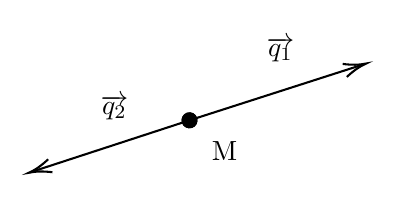
\begin{tikzpicture}[x=0.75pt,y=0.75pt,yscale=-1,xscale=1]
%uncomment if require: \path (0,92); %set diagram left start at 0, and has height of 92
%Straight Lines [id:da19898209267326417] 
\draw    (326.16,55.24) -- (409.47,28.47) ;
\draw [shift={(411.37,27.86)}, rotate = 522.19] [color={rgb, 255:red, 0; green, 0; blue, 0 }  ][line width=0.75]    (10.93,-3.29) .. controls (6.95,-1.4) and (3.31,-0.3) .. (0,0) .. controls (3.31,0.3) and (6.95,1.4) .. (10.93,3.29)   ;
\draw [shift={(326.16,55.24)}, rotate = 342.19] [color={rgb, 255:red, 0; green, 0; blue, 0 }  ][fill={rgb, 255:red, 0; green, 0; blue, 0 }  ][line width=0.75]      (0, 0) circle [x radius= 3.35, y radius= 3.35]   ;
%Straight Lines [id:da5450424757830004] 
\draw    (326.16,55.24) -- (250.59,79.91) ;
\draw [shift={(248.69,80.53)}, rotate = 341.91999999999996] [color={rgb, 255:red, 0; green, 0; blue, 0 }  ][line width=0.75]    (10.93,-3.29) .. controls (6.95,-1.4) and (3.31,-0.3) .. (0,0) .. controls (3.31,0.3) and (6.95,1.4) .. (10.93,3.29)   ;
\draw [shift={(326.16,55.24)}, rotate = 161.92] [color={rgb, 255:red, 0; green, 0; blue, 0 }  ][fill={rgb, 255:red, 0; green, 0; blue, 0 }  ][line width=0.75]      (0, 0) circle [x radius= 3.35, y radius= 3.35]   ;
% Text Node
\draw (343,70) node   [align=left] {M};
% Text Node
\draw (370,21) node    {$\overrightarrow{q_{1}}$};
% Text Node
\draw (290,49) node    {$\overrightarrow{q_{2}}$};
\end{tikzpicture}
\end{center}

We don't impose a priori conservation of momentum since it's imposed by the delta function.
\begin{gather}
p = (M, 0) \qquad
q_1 = (\omega_1, \vec{q_1}) \qquad
q_2 = (\omega_2, q_2) \notag \\
\de \Phi_{(2)} = (2 \pi)^4 \delta^4 \underbrace{(P_i - P_f)}_{= p - q_1 - q_2}
	\frac{\de^3 q_1}{(2 \pi)^3 2 \omega_1} \frac{\de^3 q_2}{(2 \pi)^3 2 \omega_2} \notag
\end{gather}
I have 6 integration parameters, 4 constraint given by $\delta^4$, so I have 2 independent variables. Integrating over $\de^3 q_2$
\[
\de \Phi'_{(2)} = \int \de \Phi_{(2)} = \frac{1}{(2 \pi)^2} \delta(M - \omega_1 - \omega_2) \frac{1}{4 \omega_1 \omega_2} \de^3 q_1
\]
in this way, the condition $\vec{q_2} = \vec{q_1}$ vanish. We have to impose it again when we calculate $\de \Gamma$ (we omit this detail)\\
Usually the 4-th non independent parameter is eliminated by integration over modulus of $q_1$, leaving free 2 parameters for the angles. 
$\de^3 q_1 \to \vec{q_1}^2 \de \abs{\vec{q_2}}\de \Omega_1$.\\ \\
Notice that $M -\omega_1 - \omega_2 = M - \sqrt{\vec{q_1}^2 + m_1^2} - \sqrt{\vec{q_2} + m_2^2}$ and then the $\delta$ implies
\[
\hat{q_1}^2 = \frac{1}{2M} \biggl( M^4 - 2M^2(m_1^2 + m_2^2) + (m_1^2 - m_2^2)^2 \biggr)^{1/2}
\]
$\abs{\vec{q_1}}$ is the only zero of $f(\abs{\hat{q_1}}) = M - \omega_1 - \omega_2$.\\
We also have
\[
\abs{f'(\abs{\hat{q_1}})} = \frac{\partial \omega_1}{\partial \abs{\vec{q_1}}} 
	+ \frac{\partial \omega_2}{\partial \abs{\vec{q_1}}} 
	= \abs{\hat{q_1}} \biggl ( \frac{\omega_1 + \omega_2}{\omega_1 \omega_2} \biggr)
\]
Using
\[
\delta \bigl( f(x) \bigr) = \sum_{x_0 = \textup{zero of f(x)}} \frac{\delta (x - x_0)}{\abs{f'(x_0)}} 
\]
and performing integration over $\de \abs{\vec{q_1}}$ we obtain
\[
\de \Phi''_{(2)} = \int \de \Phi'_{(2)} = \frac{1}{16 \pi^2} \frac{\abs{\hat{q_1}}}{M} \de \Omega_1
\]
Using this result we obtain the $1 \to 2$ decay rate in function of the solid angle (in the rest frame)
\[
\biggl( \frac{\de \Gamma_{RF}}{\de \Omega} \biggr) = \frac{1}{64 \pi^4 M^3}
	\bigl[ M^4 - 2M^2 (m_1^2 + m_2^2) + (m_1 - m_2^2)^2 \bigr]^{1/2} \abs{\mathM_{RF}}^2
\]
In a general frame we can easily obtain an analogous formula, just consider $\de \Gamma = 1/(2 \omega_in) \abs{\mathM_{fi}}^2 \de \Phi_{(nf)}$ in a general frame. remember that $\de I_{(nf)}$ is invariant \\ \\
We have 2 important limit cases:
\begin{enumerate}[label=(\Alph*)]
\item If $m_1 = m_2 = m$ (for example $Z \to e^+ e^-$)
	\begin{gather}
	\abs{\hat{q_1}} = \frac{M}{2} \biggl( 1 - \frac{4 m^2}{M^2} \biggr)^{1/2} \notag \\
	\biggl( \frac{\de \Gamma_{RF}}{\de \Omega} \biggr) = \frac{1}{64 \pi^2 M} \biggl( 1 - \frac{4 m^2}{M^2} \biggl)^{1/2} \abs{\mathM_{fi}}^2 \notag
	\end{gather}
\item If $m_1 = m, m_2 = 0$ (for example $W^{\pm} \to e^{\pm} \stackrel{(-)}{\nu}$)
	\begin{gather}
	\abs{\hat{q_1}} = \frac{M}{2} \biggl( 1 - \frac{4 m^2}{M^2} \biggr)^{1/2} \notag \\
	\biggl( \frac{\de \Gamma_{RF}}{\de \Omega} \biggr) = \frac{1}{64 \pi^2 M} \biggl( 1 - \frac{m^2}{M^2} \biggr)^{1/2} \abs{\mathM_{fi}}^2 \notag
	\end{gather}
\end{enumerate}
\textbf{Notes:} If we have two identical particles in the final state, the calculation of the phase is different
\[
\de \Phi_{(2)}^{\textup{identical}} = \frac{1}{2} \de \Phi_{(2)}^{\textup{distinguishable}}
\]
\end{example}

\section{Cross section ($\leftrightarrow$ scattering process)}

\begin{center}
\tikzset{every picture/.style={line width=0.75pt}} %set default line width to 0.75pt        

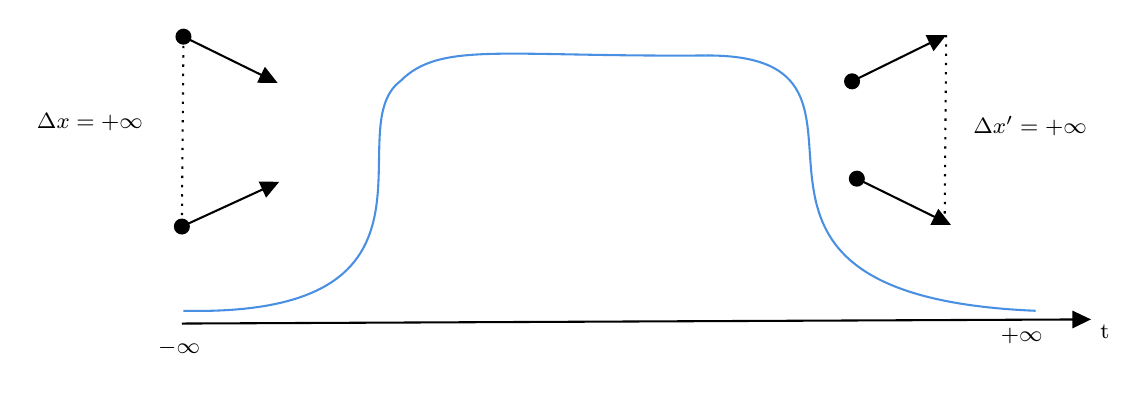
\begin{tikzpicture}[x=0.75pt,y=0.75pt,yscale=-1,xscale=1]
%uncomment if require: \path (0,300); %set diagram left start at 0, and has height of 300
%Straight Lines [id:da7420481005024371] 
\draw    (105.3,244) -- (540.3,242.01) ;
\draw [shift={(543.3,242)}, rotate = 539.74] [fill={rgb, 255:red, 0; green, 0; blue, 0 }  ][line width=0.08]  [draw opacity=0] (8.93,-4.29) -- (0,0) -- (8.93,4.29) -- cycle    ;
%Curve Lines [id:da9551272323068936] 
\draw [color={rgb, 255:red, 74; green, 144; blue, 226 }  ,draw opacity=1 ]   (106.07,237.85) .. controls (242.92,240.92) and (179.87,150.21) .. (210.63,127.14) .. controls (229.85,107.92) and (259.83,115.61) .. (357.47,114.84) ;
%Curve Lines [id:da42326511684010204] 
\draw [color={rgb, 255:red, 74; green, 144; blue, 226 }  ,draw opacity=1 ]   (357.47,114.84) .. controls (465.87,114.07) and (332.87,230.16) .. (516.61,237.85) ;
%Straight Lines [id:da05972058678475589] 
\draw    (105.3,197.26) -- (149.47,176.98) ;
\draw [shift={(152.2,175.73)}, rotate = 515.3399999999999] [fill={rgb, 255:red, 0; green, 0; blue, 0 }  ][line width=0.08]  [draw opacity=0] (8.93,-4.29) -- (0,0) -- (8.93,4.29) -- cycle    ;
\draw [shift={(105.3,197.26)}, rotate = 335.34] [color={rgb, 255:red, 0; green, 0; blue, 0 }  ][fill={rgb, 255:red, 0; green, 0; blue, 0 }  ][line width=0.75]      (0, 0) circle [x radius= 3.35, y radius= 3.35]   ;
%Straight Lines [id:da19744292721120105] 
\draw    (106.07,105.77) -- (148.74,126.74) ;
\draw [shift={(151.43,128.06)}, rotate = 206.18] [fill={rgb, 255:red, 0; green, 0; blue, 0 }  ][line width=0.08]  [draw opacity=0] (8.93,-4.29) -- (0,0) -- (8.93,4.29) -- cycle    ;
\draw [shift={(106.07,105.77)}, rotate = 26.18] [color={rgb, 255:red, 0; green, 0; blue, 0 }  ][fill={rgb, 255:red, 0; green, 0; blue, 0 }  ][line width=0.75]      (0, 0) circle [x radius= 3.35, y radius= 3.35]   ;
%Straight Lines [id:da041960146044850655] 
\draw    (430.5,174.19) -- (473.17,195.16) ;
\draw [shift={(475.86,196.49)}, rotate = 206.18] [fill={rgb, 255:red, 0; green, 0; blue, 0 }  ][line width=0.08]  [draw opacity=0] (8.93,-4.29) -- (0,0) -- (8.93,4.29) -- cycle    ;
\draw [shift={(430.5,174.19)}, rotate = 26.18] [color={rgb, 255:red, 0; green, 0; blue, 0 }  ][fill={rgb, 255:red, 0; green, 0; blue, 0 }  ][line width=0.75]      (0, 0) circle [x radius= 3.35, y radius= 3.35]   ;
%Straight Lines [id:da12165440948384254] 
\draw    (428.2,127.3) -- (470.87,106.32) ;
\draw [shift={(473.56,105)}, rotate = 513.8199999999999] [fill={rgb, 255:red, 0; green, 0; blue, 0 }  ][line width=0.08]  [draw opacity=0] (8.93,-4.29) -- (0,0) -- (8.93,4.29) -- cycle    ;
\draw [shift={(428.2,127.3)}, rotate = 333.82] [color={rgb, 255:red, 0; green, 0; blue, 0 }  ][fill={rgb, 255:red, 0; green, 0; blue, 0 }  ][line width=0.75]      (0, 0) circle [x radius= 3.35, y radius= 3.35]   ;
%Straight Lines [id:da8920203927682981] 
\draw  [dash pattern={on 0.84pt off 2.51pt}]  (106.07,105.77) -- (105.3,197.26) ;
%Straight Lines [id:da4995443342345991] 
\draw  [dash pattern={on 0.84pt off 2.51pt}]  (473.56,105) -- (472.79,196.49) ;
% Text Node
\draw (61,147) node  [font=\footnotesize]  {$\Delta x=+\infty $};
% Text Node
\draw (514,149) node  [font=\footnotesize]  {$\Delta x'=+\infty $};
% Text Node
\draw (550,248) node   [align=left] {{\footnotesize t}};
% Text Node
\draw (104,256) node  [font=\footnotesize]  {$-\infty $};
% Text Node
\draw (510,250) node  [font=\footnotesize]  {$+\infty $};
\end{tikzpicture}
\end{center}

\textbf{Scattering in the lab frame}

\begin{center}
\tikzset{every picture/.style={line width=0.75pt}} %set default line width to 0.75pt        
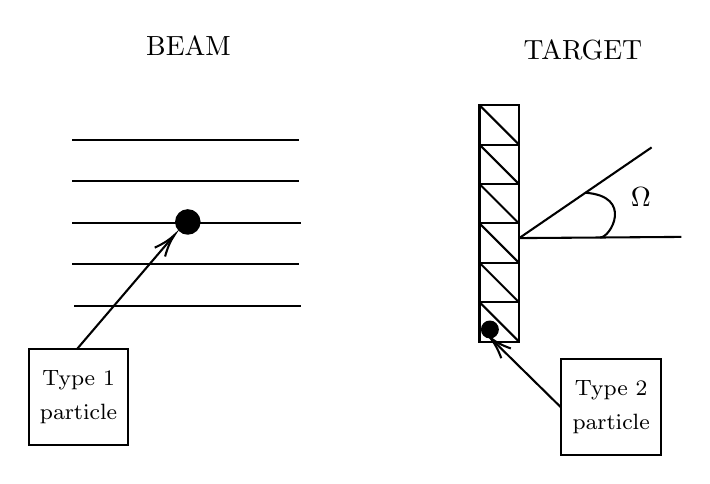
\begin{tikzpicture}[x=0.75pt,y=0.75pt,yscale=-1,xscale=1]
%uncomment if require: \path (0,300); %set diagram left start at 0, and has height of 300
%Straight Lines [id:da7601078847096199] 
\draw    (90,80) -- (199.3,80) ;
%Straight Lines [id:da41431446732450006] 
\draw    (90,100) -- (199.3,100) ;
%Straight Lines [id:da7406610884448859] 
\draw    (90,120) -- (200.3,120) ;
%Straight Lines [id:da5555389414112442] 
\draw    (90,140) -- (199.3,140) ;
%Straight Lines [id:da7113604441316939] 
\draw    (91,160) -- (200.3,160) ;
%Shape: Circle [id:dp6032562484660473] 
\draw  [fill={rgb, 255:red, 0; green, 0; blue, 0 }  ,fill opacity=1 ] (140,119.6) .. controls (140,116.48) and (142.53,113.95) .. (145.65,113.95) .. controls (148.77,113.95) and (151.3,116.48) .. (151.3,119.6) .. controls (151.3,122.72) and (148.77,125.25) .. (145.65,125.25) .. controls (142.53,125.25) and (140,122.72) .. (140,119.6) -- cycle ;
%Straight Lines [id:da4553990376870143] 
\draw    (92.3,180.8) -- (138,127.32) ;
\draw [shift={(139.3,125.8)}, rotate = 490.52] [color={rgb, 255:red, 0; green, 0; blue, 0 }  ][line width=0.75]    (10.93,-3.29) .. controls (6.95,-1.4) and (3.31,-0.3) .. (0,0) .. controls (3.31,0.3) and (6.95,1.4) .. (10.93,3.29)   ;
%Shape: Square [id:dp6385245267322448] 
\draw   (286.2,158.26) -- (305.18,158.26) -- (305.18,177.23) -- (286.2,177.23) -- cycle ;
%Straight Lines [id:da048366194956986464] 
\draw    (286.2,158.26) -- (305.18,177.23) ;
%Shape: Rectangle [id:dp3214112118743824] 
\draw   (286.2,139.28) -- (305.18,139.28) -- (305.18,158.26) -- (286.2,158.26) -- cycle ;
%Straight Lines [id:da08317295232905786] 
\draw    (286.2,139.28) -- (305.18,158.26) ;
%Shape: Square [id:dp9323954113559714] 
\draw   (286.2,120.3) -- (305.18,120.3) -- (305.18,139.28) -- (286.2,139.28) -- cycle ;
%Straight Lines [id:da45254561705281793] 
\draw    (286.2,120.3) -- (305.18,139.28) ;
%Shape: Rectangle [id:dp12155363507098405] 
\draw   (286.2,101.33) -- (305.18,101.33) -- (305.18,120.3) -- (286.2,120.3) -- cycle ;
%Straight Lines [id:da8476758996401002] 
\draw    (286.2,101.33) -- (305.18,120.3) ;
%Shape: Rectangle [id:dp34942394137534416] 
\draw   (286.2,82.35) -- (305.18,82.35) -- (305.18,101.33) -- (286.2,101.33) -- cycle ;
%Straight Lines [id:da38815018499337417] 
\draw    (286.2,82.35) -- (305.18,101.33) ;
%Shape: Ellipse [id:dp6086410383693974] 
\draw  [fill={rgb, 255:red, 0; green, 0; blue, 0 }  ,fill opacity=1 ] (287.37,171.42) .. controls (287.37,169.31) and (289.08,167.6) .. (291.19,167.6) .. controls (293.3,167.6) and (295.01,169.31) .. (295.01,171.42) .. controls (295.01,173.52) and (293.3,175.23) .. (291.19,175.23) .. controls (289.08,175.23) and (287.37,173.52) .. (287.37,171.42) -- cycle ;
%Shape: Rectangle [id:dp006552695566079958] 
\draw   (286.2,63.37) -- (305.18,63.37) -- (305.18,82.35) -- (286.2,82.35) -- cycle ;
%Straight Lines [id:da9936025699051918] 
\draw    (286.2,63.37) -- (305.18,82.35) ;
%Straight Lines [id:da19771769575127984] 
\draw    (325.3,208.8) -- (292.61,176.64) ;
\draw [shift={(291.19,175.23)}, rotate = 404.53999999999996] [color={rgb, 255:red, 0; green, 0; blue, 0 }  ][line width=0.75]    (10.93,-3.29) .. controls (6.95,-1.4) and (3.31,-0.3) .. (0,0) .. controls (3.31,0.3) and (6.95,1.4) .. (10.93,3.29)   ;
%Straight Lines [id:da661445200042976] 
\draw    (305.34,127.38) -- (383.4,126.81) ;
%Straight Lines [id:da0566268996079935] 
\draw    (305.34,127.38) -- (369.12,83.68) ;
%Curve Lines [id:da8769720720143497] 
\draw    (337.23,105.53) .. controls (360.55,107.24) and (349.37,127.1) .. (344.37,127.1) ;
% Text Node
\draw    (69,181) -- (117,181) -- (117,227) -- (69,227) -- cycle  ;
\draw (93,204) node   [align=center] {{{\footnotesize Type 1}}\\{{\footnotesize particle}}};
% Text Node
\draw (146,35) node   [align=center] {{BEAM}};
% Text Node
\draw    (325.62,185.8) -- (373.62,185.8) -- (373.62,231.8) -- (325.62,231.8) -- cycle  ;
\draw (349.62,208.8) node   [align=center] {{{\footnotesize Type 2}}\\{{\footnotesize particle}}};
% Text Node
\draw (363.9,107.39) node    {$\Omega $};
% Text Node
\draw (336,37) node   [align=left] {TARGET};
\end{tikzpicture}
\end{center}

Consider a beam of particles with mass $m_1$, number (assuming a uniform distribution) density $n_1^{(0)}$ (subscript 0 is meant to stress that these are number densities in a specific frame, that with particle 2 at rest) and velocity $v_1$ inpining on a target made of particles with mass $m_2$ and number density $n_2^{(0)}$ at rest.\\
Let $N_s$ be the number of scattering events that place per unit volume and per unit time
\[
\frac{N_t}{T} \phi_1 N_2 \sigma = \bigl( n_1^{(0)} v_1 \bigr) \bigl( n_2^{(0)} V \bigr) \sigma
\]
More formally we have
\[
\de N_s = \sigma v_1 n_1^{(0)} n_2^{(0)} \ \de V \de V
\]
with:
\begin{enumerate}
\item T: unit of time
\item $\phi_1$: flux of the beam $\phi_1 = n_1^{(0)} v_1$
\item $N_2$: particles per unit volume in the detector $N_2 = n_2^{(0)}V$
\item $\sigma$: proportionality constant
\end{enumerate}
Dimensional analysis shows $[\sigma] = [L]^2$ and then $\sigma$, called cross section, can be interpreted as an ``effective area''\\
Consider the case where just one particle collides with another particle (2 particles scattering). We can obtain this condition imposing $n_{1,2}^{(0)} = 1/V$, in this way the scattering per unit of volume is the same as two particles scattering\\
Notice that this situation is the more physical. The probability of 3 particles collision in the same $\de^3 x$ and $\de t$ is almost 0\\ \\
If $\de \omega$ is, again, the probability for a process in which in the final state the i-th particle has momentum between $p_i$ and $p_i + \de p_i$
\[
\de \omega = (2 \pi)^4 \delta^4 (p_i - p_f) VT \biggl( \frac{1}{2 \omega_1 V} \biggl) \biggl( \frac{1}{2 \omega_2 V} \biggr) \
	\prod_{l=1}^{n_f} \biggl( \frac{\de^3 pl}{(2 \pi)^3 2 \omega_l} \biggr) \abs{\mathM_{fi}}^2
\]
we can define the \textbf{differential cross section} (in the lab frame) \textbf{$\de \sigma$} as
\[
\begin{split}
(\de \sigma)_{\textup{LAB}}	& = \frac{\de \omega}{n_1^{(0)} n_2^{(0)} v_1 VT}	\\
						& =\frac{V}{T v_1} \de \omega \\
						& = (2 \pi)^4 \delta^4 (p_i - p_f) \
						\prod_{l_1}^{n_f} \biggl( \frac{\de^3 p_l}{(2 pi)^3 2 \omega_l} \biggr)
						\frac{\abs{\mathM_{fi}}^2}{4 \omega_1 \omega_2 v_1}
						\qquad \textup{with } \omega_2 = m_2
\end{split}
\]
The result is then
\[
(\de \sigma)_{\textup{LAB}} = \frac{1}{4 \omega_1 v_1 m_2} \abs{\mathM_{fi}}^2 \ \de \Phi_{(nf)}
\]
All quantities refers to the rest frame for particle 2 ($\omega_1 = \omega_1^{(0)}, v_1 = v_1^{(0)}$)\\
In order to obtain a covariant relation for $\de \sigma$, we notice that the only non-covariant factor in the latter relation is $(I_{12})_{\textup{LAB}} = \omega_1^{(0)} m_2$. This factor can be substituted with a covariant one
\[
I_{12} = \bigl[ (p_1 p_2)^2 - m_1^2 m_2^2 \bigr]^{1/2}
\]
called \textbf{covariant flux factor}. This factor is obviously covariant, we just have to prove that in the lab frame it coincides with $(I_{12})_{\textup{LAB}}$.
In the lab frame we have $p_1 = (\omega_1, \vec{p_1}^{(0)})$ and $p_2 = (m_2, \vec{0})$, so the previous formula becomes
\[
\bigl[ m_2^2 (\omega_1^{(0)})^2 - m_1 m_2 \bigr]^{1/2} = m_2 \bigl( (\omega_1^{(0)})^2 - p_1^2 \bigr)^{1/2} = m_2 \abs{\vec{p_1^{(0)}}}
	= m_2 \omega_1^{(0)} v_1^{(0)}
\]
So the final result is
\[
\de \sigma = \frac{\abs{\mathM_{fi}^2}}{4 I_{12}} \de \ \Phi_{(nf)}
\]

\newpage
\begin{example}[$2 \to 2$ scattering]
Consider a scattering process $2 \to 2$. We consider an initial state with two particles with masses $m_1, m_2$ and four momenta $p_1, p_2$ and a final state with masses $m'_1, m'_2$ and four momenta $p'_1, p'_2$

\begin{center}
% Pattern Info
\tikzset{
pattern size/.store in=\mcSize, 
pattern size = 5pt,
pattern thickness/.store in=\mcThickness, 
pattern thickness = 0.3pt,
pattern radius/.store in=\mcRadius, 
pattern radius = 1pt}
\makeatletter
\pgfutil@ifundefined{pgf@pattern@name@_hj3mih7tf}{
\pgfdeclarepatternformonly[\mcThickness,\mcSize]{_hj3mih7tf}
{\pgfqpoint{0pt}{0pt}}
{\pgfpoint{\mcSize+\mcThickness}{\mcSize+\mcThickness}}
{\pgfpoint{\mcSize}{\mcSize}}
{
\pgfsetcolor{\tikz@pattern@color}
\pgfsetlinewidth{\mcThickness}
\pgfpathmoveto{\pgfqpoint{0pt}{0pt}}
\pgfpathlineto{\pgfpoint{\mcSize+\mcThickness}{\mcSize+\mcThickness}}
\pgfusepath{stroke}
}}
\makeatother
\tikzset{every picture/.style={line width=0.75pt}} %set default line width to 0.75pt        
\begin{tikzpicture}[x=0.75pt,y=0.75pt,yscale=-1,xscale=1]
%uncomment if require: \path (0,300); %set diagram left start at 0, and has height of 300
%Shape: Ellipse [id:dp21530724204661533] 
\draw  [pattern=_hj3mih7tf,pattern size=6pt,pattern thickness=0.75pt,pattern radius=0pt, pattern color={rgb, 255:red, 0; green, 0; blue, 0}] (325.39,126.56) .. controls (325.39,118.14) and (332.22,111.32) .. (340.63,111.32) .. controls (349.05,111.32) and (355.87,118.14) .. (355.87,126.56) .. controls (355.87,134.97) and (349.05,141.79) .. (340.63,141.79) .. controls (332.22,141.79) and (325.39,134.97) .. (325.39,126.56) -- cycle ;
%Straight Lines [id:da9191843337533081] 
\draw    (255.3,95.8) -- (326.45,121.53) ;
%Straight Lines [id:da8608860797521036] 
\draw    (355.44,130.25) -- (424.89,156.58) ;
%Straight Lines [id:da7041811863832155] 
\draw    (255.3,157.8) -- (326.19,131.02) ;
%Straight Lines [id:da585605593647289] 
\draw    (355.18,122.04) -- (425.5,96.41) ;
% Text Node
\draw (240,87) node  [font=\footnotesize]  {$p_{1}$};
% Text Node
\draw (239,162) node  [font=\footnotesize]  {$p_{2}$};
% Text Node
\draw (436,93) node  [font=\footnotesize]  {$p'_{1}$};
% Text Node
\draw (436,157) node  [font=\footnotesize]  {$p'_{2}$};
\end{tikzpicture}
\end{center}
With
\[
p_1 = (\omega_1, \vec{p_1}) \qquad
p_2 = (\omega_2, \vec{p_2}) \qquad
p'_1 = (\omega'_1, \vec{p'_1}) \qquad
p'_2 = (\omega'_2, \vec{p'_2})
\]
With a procedure identical to $1 \to 1$ decay (imposing also $\vec{p'_2} = \vec{p_1} + \vec{p_2} - \vec{p'_1}$ when we calculate $\de \sigma$), we obtain 
\[
\de \Phi'_{(2)} = \frac{1}{(2 \pi)^2} \frac{1}{4 \omega'_1 \omega'_2} \delta (\omega_1 + \omega_2 - \omega'_1 - \omega'_2) \ \de^3p'_1
\]
In order to integrate over $\de \abs{\vec{p'_1}}$ it is useful to introduce Mandelstam variables s, t and u
\[
s = (p1 + p2)^2 \qquad
t = (p1 - p'_1)^2 \qquad
u = (p_1 - p'_2)^2
\]
These variables are clearly Lorentz invariants, and satisfy (using $p_1 + p_2 = p'_1 + p'_2$) the relation
\[
s + t + u = m_1^2 + m_2^2 + (m'_1)^2 + (m'_2)^2
\]
It is useful to work in the center of mass frame, where the incoming particles have $p_1 = (\omega_1, \vec{p})$ and $p_2 = (\omega_2, -\vec{p})$. Computing s in the CM frame we obtain $s = (\omega_1 + \omega_2)^2 = (\omega'_1 + \omega'_2)^2$ and then
\begin{gather}
p_1 + p_2 = (\sqrt{s}, 0) \notag \\
\delta(\omega_1 + \omega_2 - \omega'_1 -\omega'_2) = \delta (\sqrt{s} - \omega'_1 - \omega'_2) \notag
\end{gather}
With a procedure identical to the one used for $1 \to 2$ decay ($M \leftrightarrow \sqrt{s}$) we obtain
\begin{gather}
\bigl( \de \Phi''_{(2)} \bigr)_{CM} = \frac{1}{16 \pi^2} \frac{\abs{\widehat{p'_1}}_{CM}}{\sqrt{s}} \ \de \Omega'_1 \notag \\
\abs{\widehat{p'_1}}_{CM} = \frac{1}{2 \sqrt{s}} \biggl[ s^2 + (m^{\prime 2}_1 + m^{\prime 2}_2)^2 - 2s (m^{\prime 2}_1 + m^{\prime 2}_2) \biggr]^{1/2} \notag
\end{gather}
The covariant flux factor in CM frame reads
\[
(I_{12})_{CM} = \bigl[ \vec{p}^2 (\omega_1 + \omega_2 )^2 \bigr]^{1/2} = \abs{\vec{p}} \sqrt{s}
\]
So we obtain the final result
\[
\begin{split}
\biggl( \frac{\de \sigma}{\de \Omega'_1} \biggr)_{CM} 	
	& = \frac{1}{64 \pi^2 s} \frac{\abs{\widehat{p'_1}}_{CM}}{\abs{\vec{p}}} \ \abs{\mathM_{fi}}^2_{CM} \\
	& = \frac{1}{128 \pi^2 s^{3/2}} \frac{1}{\abs{\vec{p}}}
		\bigl[s^2 + (m_1^{\prime 2} - m_2^{\prime 2})^2 - 2s(m_1^{\prime 2} + m_2^{\prime 2}) \bigr]^{1/2}
		\abs{\mathM_{fi}}^2_{CM}
\end{split}
\]
We have two important limit cases
\begin{enumerate}[label=(\Alph*)]
\item If $m_1 = m'_1, m_2 = m'_2$, i. e. elastic scattering (for example $e^- \mu^{\dagger} \to e^-\mu^{\dagger}$)
	\begin{equation*}
	\left. \begin{aligned}
	\abs{\vec{p_1}} = \abs{\vec{p'_1}}, \omega_1 = \omega'_1 \\
	\abs{\vec{p_2}} = \abs{\vec{p'_2}}, \omega_2 = \omega'_2
	\end{aligned}
	\right \}
	\quad \abs{\hat{p'_1}}_{CM} = \abs{\vec{p}}
	\end{equation*}
	\[
	\Biggl( \frac{\de \sigma}{\de \Omega'_1} \Biggr)_{CM} = \ \frac{1}{64 \pi^2} \frac{\abs{\mathM_{fi}}^2}{s}
	\]
\item If $m_1 = m_2 \simeq 0, m'_1 = m'_2 = M$ (for example $e^-e^+ \to \mu^- \mu^+$)
	\begin{gather}
	\abs{\vec{p_1}} = \abs{\vec{p}}, \omega_1 = \frac{\sqrt{s}}{2} \notag \\
	\abs{\hat{p'_1}} = \frac{\sqrt{s}}{2} \Biggl( 1 - \frac{1}{4M^2}{s} \Biggr)^{1/2} 
	\end{gather}
$4M^2/s$ processes with $s < 4M^2$ are unphysical
	\[
	\Biggl( \frac{\de \sigma}{\de \Omega'_1} \Biggr)_{CM} = \ \frac{1}{64 \pi^2} 
	\Biggl( 1 - \frac{4M^2}{s} \Biggr)
	\frac{\abs{\mathM_{fi}}^2}{s}
	\]
\end{enumerate}
\end{example}

The previous formulas are valid also for particles with spin, if the initial and final spin states are known; in this case the initial state has the form $\Ket{i} = \Ket{\vec{p_1}, \vec{s_1}; \dots; \vec{p_n}, \vec{s_n}}$, and similarly for the final state.\\
However, experimentally is more common that we do not know the initial spin configuration and we accept in the detector all final spin configurations; in this case, to compare with experiment, we must
\begin{enumerate}
\item Considering all (equally present) polarization of initial state, i.e. \textit{average} over the initial spin configuration
\item Considering all final polarizations, i.e. \textit{sum} over all possible final configurations
\end{enumerate}
Defining the \textbf{unpolarized Feynman amplitude $\overline{\abs{\mathM_{fi}}}$} as
\[
\overline{\abs{\mathM_{fi}}^2} = \frac{1}{\text{n initial polarizations}} \
	=\sum _{\text{initial spins}} \ \sum _{\text{final spins}} \ \abs{\mathcal{M}_{fi}}^{2}
\]
we just hace to substitute $\abs{\mathM_{fi}}^2 \to \abs{\mathM_{fi}}^2$ in all previous formulas\\
For example, in $2 \to 2$ scattering
\[
\frac{1}{\text{n init pol}} = \frac{1}{(2 s_a + 1)(2 s_b + 1)}
\qquad \text{where } s_a = \text{spin of particle 1; and } s_b = \text{spin of particle 2}
\]